\chapter{Electrically Detected Magnetic Resonance on a Cathode of an Organic Radical Battery}

\paragraph*{}
With EDMR we observe the hopping charge as it travels to the charge bearing group through the electrode.

\subsection{Spin Blockade and Spin-Dependent Recombination}

\subsection{Instrumentation}

\subsection{Device Fabrication}
\subsubsection{1N4007 Si diode}
A commercial 1N4007 p-n Si diode was modified to use as a standard for the EDMR experiments. The plastic housing of the diode was opened and the copper leads were etched out to reduce the metal content of the sample that strongly suppresses the $B_1$ field needed for reaching the resonance condition, and, additionally, leads to the heating of the sample which affects the current through the diode. The diode with the opened housing was placed into a droplet of concentrated nitric acid (65\% HNO$_3$) and the etching process was observed in a microscope. When the copper leads have reduced in size so that only a thin layer of copper was covering the Si crystal, the etching reaction was stopped with ethanol. Two $\oslash~0.1$~mm Ag wires were used to connect the diode to the detection circuit through the screened coaxial cables. The device was placed in a $\oslash~4.9$~mm OD quartz EPR sample tube.\\

\subsubsection{DPP-DTT Organic Ambipolar Field Effect Transistor}
An organic field-effect transistor was fabricated by Z. Wang in the Cavendish Laboratory of the University of Cambridge in a glovebox filled with Ar. A 3.5~mm wide, 1~mm thick quartz substrate was carrying two on-substrate meander-shaped Au electrodes as the drain and the source electrodes. A thin film of DPP-DTT was spin-coated on the on-substrate electrodes. A layer of ???? was spin-coated as the gate isolator on top of the DPP-DTT film. The Au gate electrode was evaporated onto the isolator layer through a shadow mask. The metal electrodes were extended with a wire bonder, and soldered to thick Cu wires. The device was encapsulated in a $\oslash~4.9$~mm OD quartz EPR sample tube.

\subsubsection{pDiTBuS Organic Radical Battery}


\subsection{EDMR signal in a 1N4007 Si Diode}




\subsection{EDMR signal in an Organic Field Effect Transistor}

\subsection{EDMR signal in a TEMPO-Salen Electrochemical Cell}


\subsection{Distribution of Current Density in On-Substrate Meander-Shaped Electrodes}
Meander-shaped electrodes shown in Figure~\ref{fig:grid} are used to study properties of thin conductive films. The distribution of electric potential and the current within a film of poor conductivity and a finite thickness be not obvious. 

\begin{figure} [!ht]
\begin{center}
       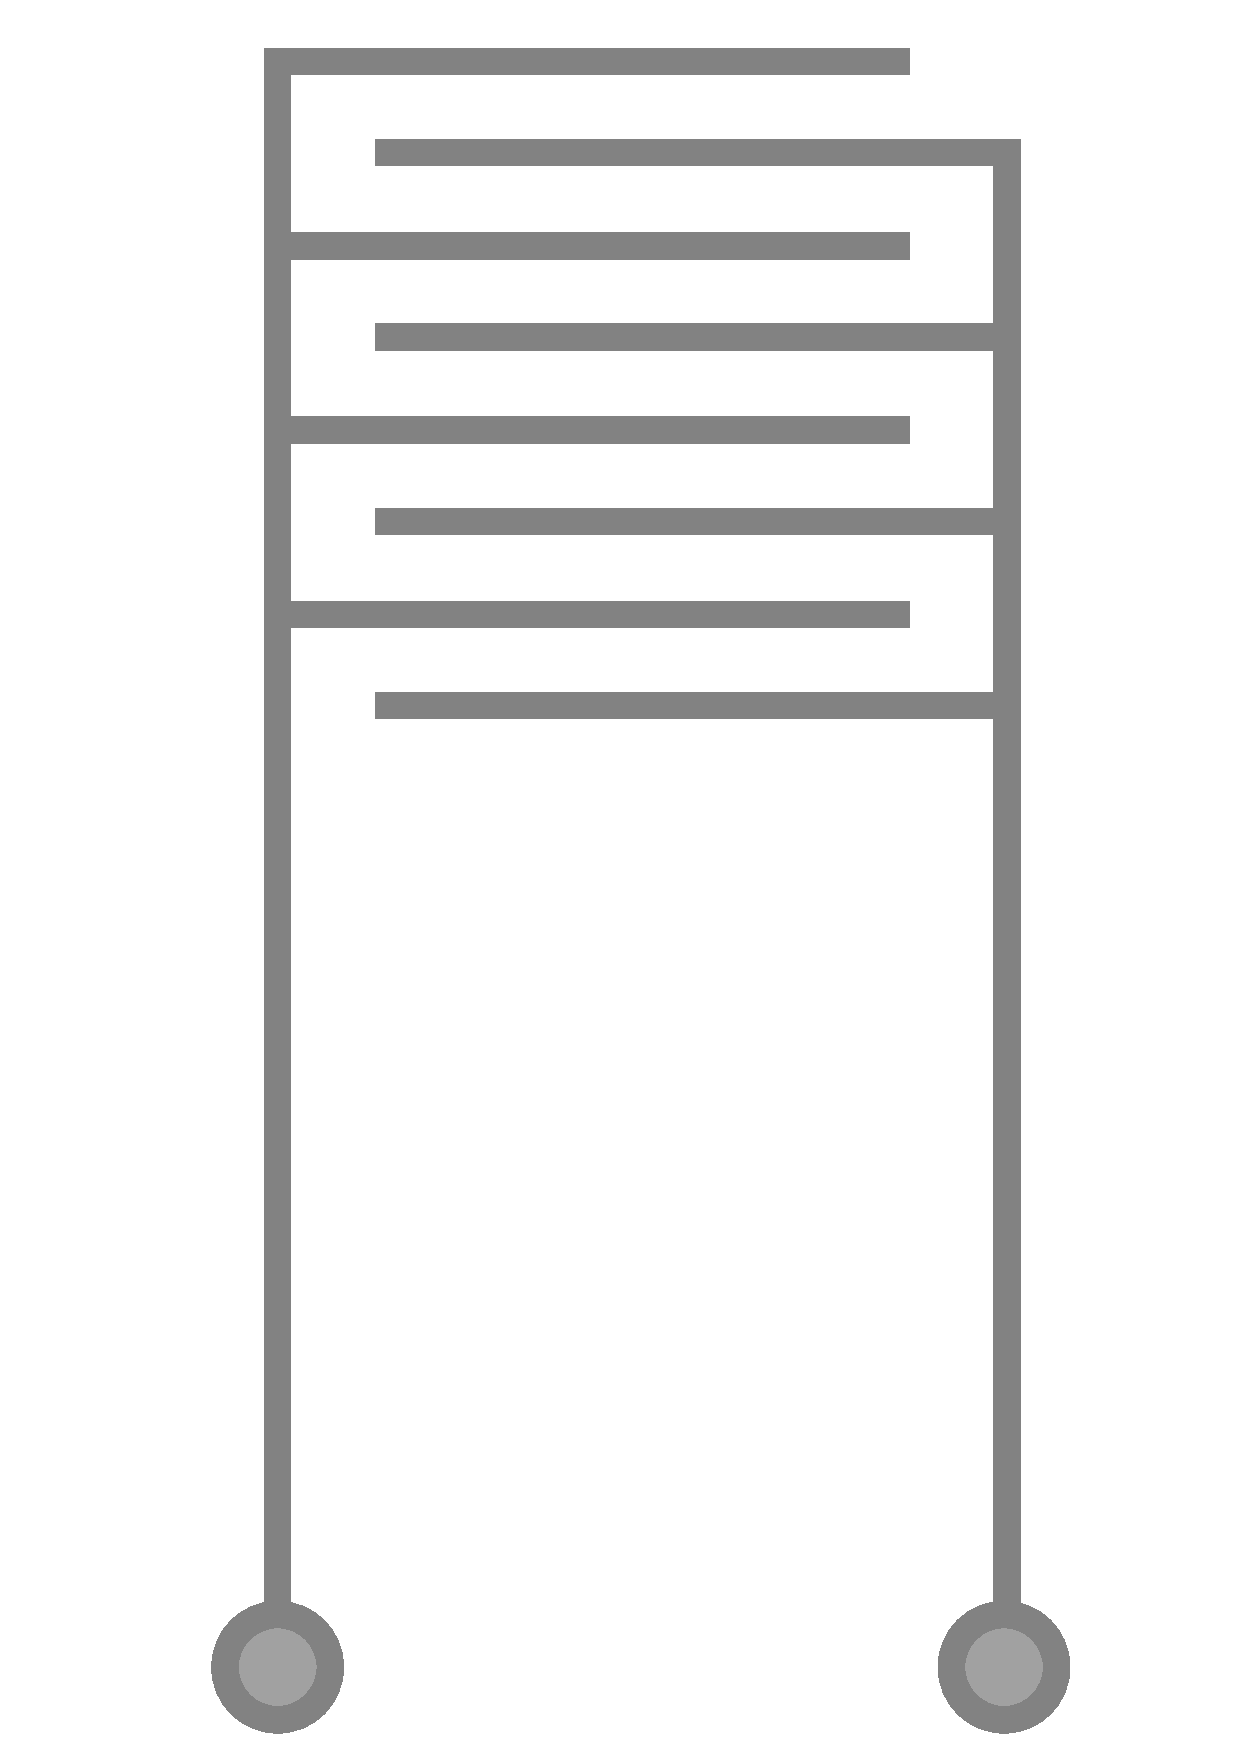
\includegraphics[width=0.5\textwidth]{./edmr/fingers1/pics/grid.pdf}
       \end{center}
\caption{Transformation of the meander-shaped electrode grid into two linear electrodes}
     \label{fig:grid}
\end{figure}

A numerical solution was found to the distribution of the current density $\vec{j}$ within a film of a finite thickness, connected by two metal electrodes. Two cases were considered, a thick film and a thin film.

\begin{figure} [!ht]
\begin{center}
       \includegraphics[width=0.5\textwidth]{./edmr/fingers1/pics/3_thick_film.png}
       \end{center}
\caption{Distribution of electric current in a thick polymer film. The current is uniform in the middle of the film. \raw{Let us see, whether we can apply the simple, bulk formula to this structure.}}
     \label{fig:dits_thick_2d}
\end{figure}

\begin{figure} [!ht]
\begin{center}
       \includegraphics[width=0.5\textwidth]{./edmr/fingers1/pics/3_thick_film_2.png}
       \end{center}
\caption{Thick film. The current is uniform in the middle of the film. It is better seen on this 3d plot. Let us see, whether we can apply the simple, bulk formula to this structure. \raw{I think we do not gain a lot of error by saying that the current is uniform within the whole film.}}
     \label{fig:dits_thick_3d}
\end{figure}


\begin{figure} [!ht]
\begin{center}
       \includegraphics[width=0.5\textwidth]{./edmr/fingers1/pics/2_intermediate_film.png}
       \end{center}
\caption{Distribution of electric current in an intermediate polymer film}
     \label{fig:dits_inter}
\end{figure}

\begin{figure} [!ht]
\begin{center}
       \includegraphics[width=0.5\textwidth]{./edmr/fingers1/pics/1_thin_film.png}
       \end{center}
\caption{Distribution of electric current in a thin polymer film}
     \label{fig:dits_thin}
\end{figure}

\begin{figure} [!ht]
\begin{center}
       \includegraphics[width=0.5\textwidth]{./edmr/fingers1/pics/3_intermediate_film_2.png}
       \end{center}
\caption{Very high values of the computed distribution of the current density in a film of intermediate thickness due to the sharp edges of the contacts.}
     \label{fig:dits_singular}
\end{figure}


